%----------------------------------------------------------------------------
\chapter{Megoldandó feladatok}\label{sect:LatexTools}
%----------------------------------------------------------------------------
A házi feladat során az alábbi feladatokat kellett elvégezni:
\begin{enumerate}
	\item Végezzék el a mellékletben leírt számítást a \textbf{Matlab PDE Toolbox}-szal, amely egy motor mágneses terének egyszerűsített modellje.
	\item Az indukcióvonalak mellett ábrázolják a mágneses indukció abszolút értékének eloszlását.
	\item Végezzék el a számítást $ \mu_{r}=5200 $ relatív permeabilitású, lineáris vas feltételezésével is, és vessék össze az eredményt az előzővel. 
	\item Hogyan változik a mágneses indukció abszolút értékének maximuma, ha finomabb végeselemhálót használnak?
\end{enumerate}
%\begin{figure}[!ht]
%	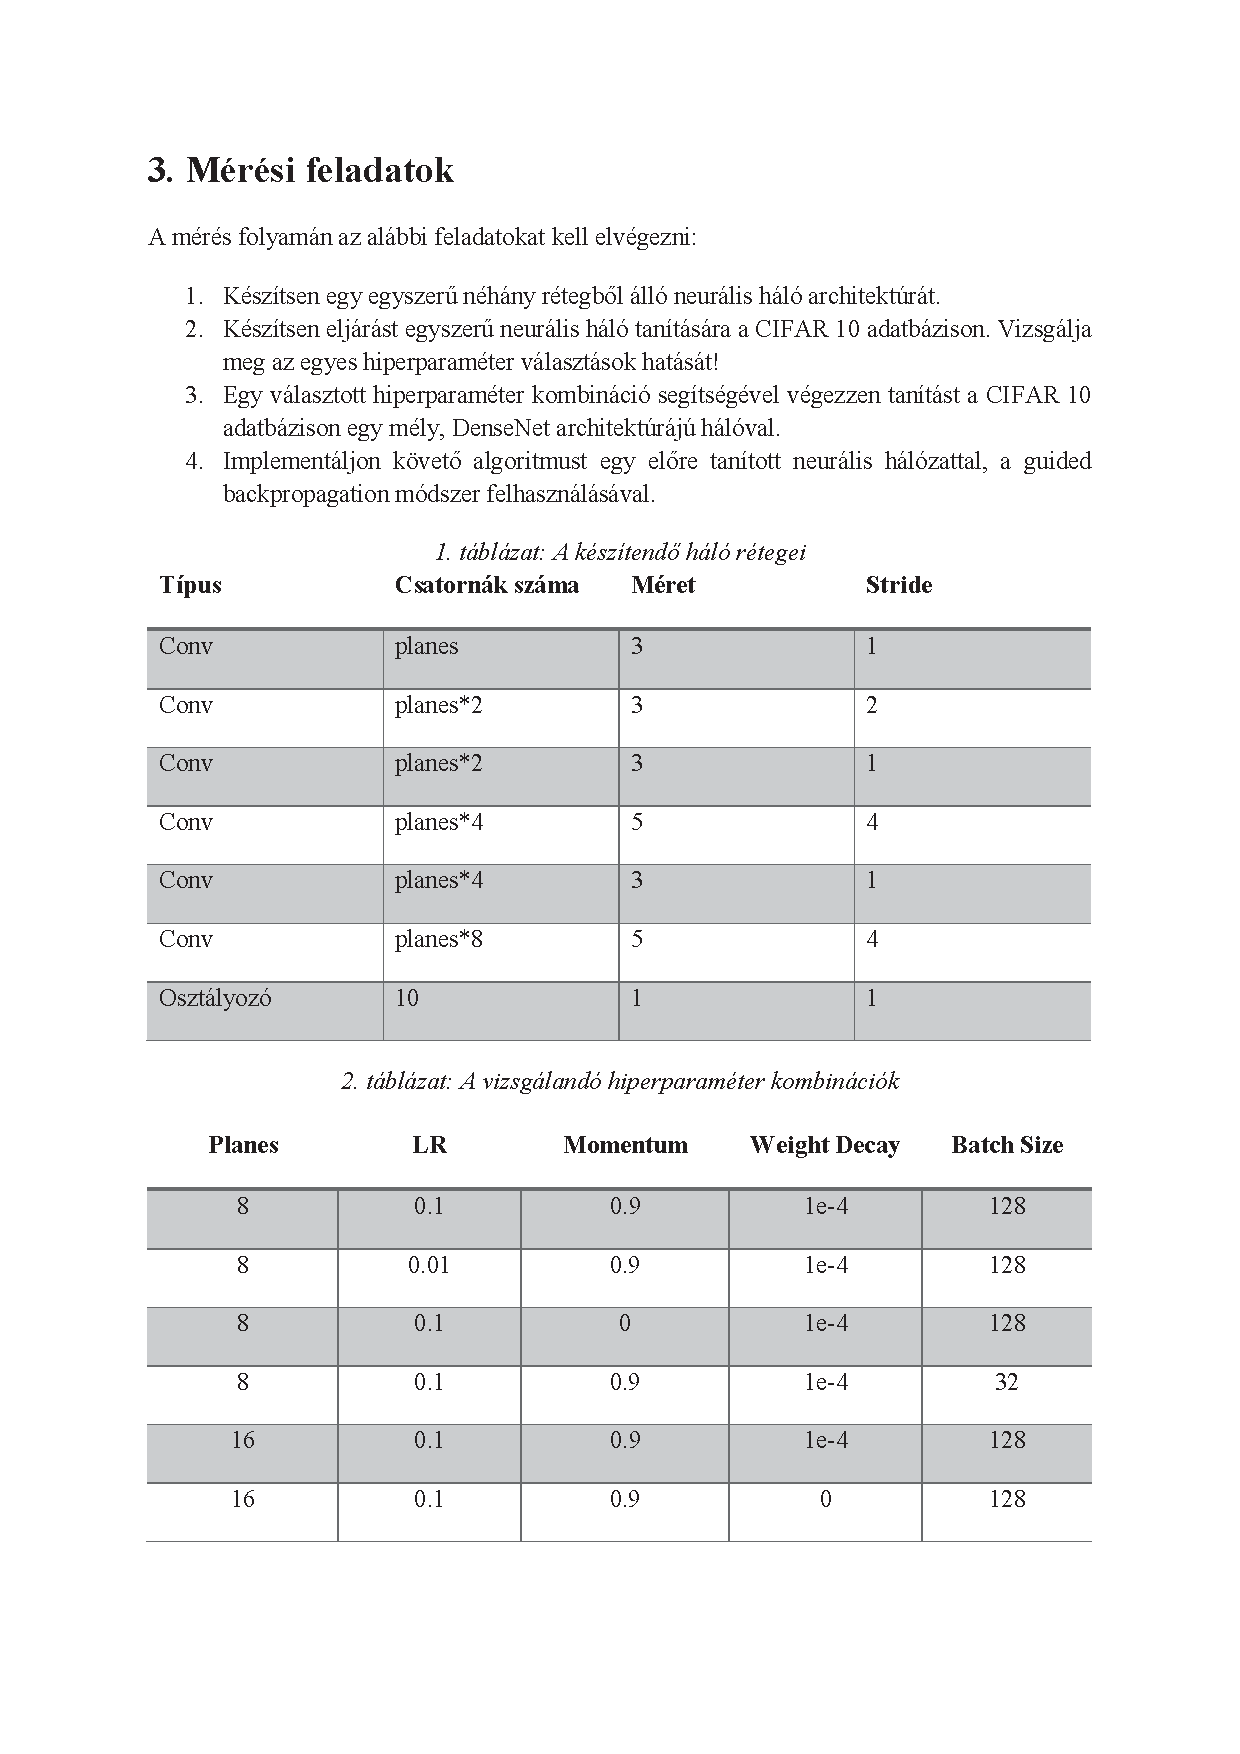
\includegraphics[trim = 25mm 210mm 20mm 33mm,clip, width=150mm,keepaspectratio]{figures/feladatok_m07.pdf}
%	\label{fig:Road-of-a-char}
%\end{figure}
